\par {\actuality} Данная работа посвящена исследованию поведения тяжёлых ионов и поляризованных пучков лёгких заряженных частиц в ускорительных и накопительных установках с целью изучения фундаментальных свойств материи. Представленные результаты направлены на формирование комплексной физической программы исследований, включающей вопросы по разрешению спинового кризиса и изучению электрического дипольного момента элементарных частиц.

\par Механизм формирования и эволюции Вселенной до сих пор остается загадкой. На ранних этапах формирования Вселенная находилась в состоянии экстремально плотной и горячей материи, известной как кварк-глюонная плазма \autocite{phase_transition_universe}. Подобное состояние материи наблюдается в недрах нейтронных звезд \autocite{neutron_stars} и в результате столкновения тяжелых заряженных частиц. Подобные эксперименты могут осуществляться в рамках коллайдерных исследований с тяжелыми частицами и помогут в изучении фазовых переходов и критических явлений в сильновзаимодействующей ядерной материи при экстремальных барионных плотностях \autocite{quark_gluon}.

\par	Для получения статистически значимых результатов в коллайдерном эксперименте необходимо накопление достаточного объёма экспериментальных данных, что количественно характеризуется интегральной величиной — светимостью. Обеспечение её высокого уровня является ключевым требованием. Для исследования кварк-глюонной плазмы светимость находится на уровне порядка $10^{27}$~$\text{см}^{-2}\cdot\text{c}^{-1}$ для тяжелоионного пучка \autocite{RHIC_luminosity_heavy}. Достижение таких рекордных значений требует тонкой настройки всех систем ускорителя, что может быть связано с большими временными затратами. При ускорении тяжёлых ионов высокая зарядность и интенсивность пучка накладывают серьёзные ограничения на параметры сгустка из-за внутрипучкового рассеяния (ВПР) \autocite{2016_IBS}. Для преодоления этих проблем, структура должна обладать высоким временем ВПР и содержать специальные установки стохастического и электронного охлаждения.

\par	Другой нерешенной проблемой современной физики остается вопрос о распределении спина внутри протона, так называемый "\textit{спиновый кризис протона}". В 1989 году коллаборация EMC (European Muon Collaboration) \autocite{spin_crisis_1989} показала, что вклад кварков в спин протона составляет небольшую часть и по оценкам находится на уровне около 30$\%$ \autocite{quarks_overview_2022}. Исследования этого вопроса проводились в коллайдерных экспериментах c использованием поляризованных протонных и дейтронных пучков: при низких энергиях -- на установках COSY-ANKE \autocite{COSY_ANKE} и SATURNE \autocite{SATURNE}, а при высоких энергиях на RHIC \autocite{RHIC_2014}. 

\par	Изучение спиновой структуры протонов и дейтронов требует подготовки и ускорения поляризованных пучков, обеспечивающих светимость порядка $10^{32}$~$\text{см}^{-2}\cdot\text{с}^{-1}$ \autocite{RHIC_luminosity}. Поляризация пучка является дополнительной степенью свободы, вследствие чего определённые сечения рассеяния приобретают зависимость от поляризации сталкивающихся сгустков. Поскольку отношение заряда к массе для протона почти в два раза отличается от соответствующего значения для тяжёлых ионов, максимальная энергия эксперимента кратно увеличивается. В структуре, оптимальной для тяжёлоионного эксперимента, критическая энергия подобрана таким образом, что столкновение происходит до достижения её значения, и, следовательно, никаких проблем с её преодолением не возникает. Критическая энергия является важным параметром ускорительной установки, и при разработке структуры этому вопросу уделяется особое внимание. Для протонов прохождение критической энергии становится ключевым фактором, ограничивающим параметры сгустка и требующим принятия дополнительных мер для её преодоления.

\par	При ускорении протонного пучка длительное нахождение вблизи критической энергии или пересечение этой области существенно влияет на параметры и стабильность пучка. В такой ситуации нарушается адиабатичность продольного движения, усиливаются нелинейные эффекты, а затухание Ландау уже не способно эффективно подавлять возникающие возмущения. Дополнительное воздействие оказывают пространственный заряд и другие импедансы, способствуя развитию продольной микроволновой неустойчивости, нестабильности отрицательной массы и поперечной неустойчивости типа «голова–хвост» (head–tail) \autocite{ng, lee}. При малой интенсивности влияние критической энергии на параметры сгустка несущественно. Проблема становится актуальной для интенсивных пучков с числом частиц порядка $10^{10}$–$10^{12}$. Высокая интенсивность в коллайдерных экспериментах определяется требованиями по достижению большой светимости, однако любое увеличение эмиттанса приводит к её снижению. Степень проявления указанных эффектов определяется временем пребывания пучка вблизи критической энергии, поэтому применяются методы быстрого пересечения или поднятия критической энергии.

\par	Известная проблема физики состоит в объяснении барионной асимметрии, то есть наблюдаемого преобладания материи над антиматерией. Существующие законы физики до сих пор не способны полностью объяснить этот дисбаланс. В работе 1967 год А. Д. Сахаров сформулировал общие необходимые условия для возникновения барионной асимметрии: 1) нарушение закона сохранения барионного заряда; 2) нарушение C- и CP-симметрии; 3) нарушение на ранних этапах формирования Вселенной термодинамического равновесия \autocite{sakharov}. Согласно второму условию, "\textit{Возникновение С-асимметрии по нашей гипотезе является следствием нарушения СР-инвариантности при нестационарных процессах расширения горячей Вселенной на сверхплотной стадии, которое проявляется в эффекте различия парциальных вероятностей зарядово-сопряженных реакций}".  Ранее, в 1958 году, С. Окубо теоретически показал наличие подобного эффекта при рассмотрении распада сигма-гиперон $\Sigma^{+}$ и его античастицы $\bar{\Sigma}^{+}$. Позднее, в 1964 году, Д. Кронин и В. Фитч экспериментально обнаружили нарушение CP-инвариантности слабого взаимодействия в распаде нейтральных каонов $K_{2}^{0}$ на два пиона $\pi^{+}, \pi^{-}$ \autocite{CP}, за что в 1980 году были удостоены Нобелевской премии по физике.

\par	В современной Стандартной модели частиц нарушаются P-\autocite{P-violation} и CP-симметрии. Источником CP-нарушения является наличие комплексной фазы в матрице смешивания кварков Кабиббо-Кабаяси-Маскавы для слабых взаимодействий \autocite{CKM} и коэффициента $\theta_{\text{QCD}}$ в лагранжиане квантовой хромодинамики \autocite{CPstrong}, однако в сильных взаимодействиях CP-нарушений не обнаружено. Согласно CPT-теореме, CP-инвариантность эквивалентна T-инвариантности. Ненулевой электрический дипольный момент (ЭДМ) элементарных частиц может быть источником такого нарушения. ЭДМ является фундаментальным свойством материи, обусловленным неоднородностью распределения заряда внутри частицы. Поскольку ЭДМ представляется полярным вектором, а не псевдовектором, для него нарушается как P-, так и T-инвариантность, что показано на рис. \ref{fig:4edmpt}. Величина ЭДМ в Стандартной модели мала для экспериментального детектирования и оценивается на уровне $\abs{d_{n}}< 10^{-30}-10^{-32}$ $e\cdot \text{см}$ для нейтрона \autocite{EMD_overview}. Возможность существования ЭДМ была впервые обсуждена в заметке Перселла и Рэмси в 1950 году \autocite{EDM}, однако ненулевой ЭДМ пока не обнаружен. Суперсимметричные теории (SUSY) предсказывают ЭДМ на уровне $\abs{d_{n}}< 10^{-27}-10^{-29}$ $e\cdot \text{см}$ для нейтрона, что создаёт реальные перспективы его экспериментального обнаружения. Такие точности не достигнуты: первые существенные ограничения были установлены Н. Рэмси и коллегами $\abs{d_{n}}< 5\times10^{-20}$ $e\cdot \text{см}$ ($90\%$ C.L.) \autocite{NeutronEDM}, а современное ограничение, полученное в эксперименте nEDM, составляет $\abs{d_{n}}< 1.8\times 10^{-26}$ $e\cdot \text{см}$ ($90\%$ C.L.) \autocite{neutron_EDM_current}.

\begin{figure}
	\centering
	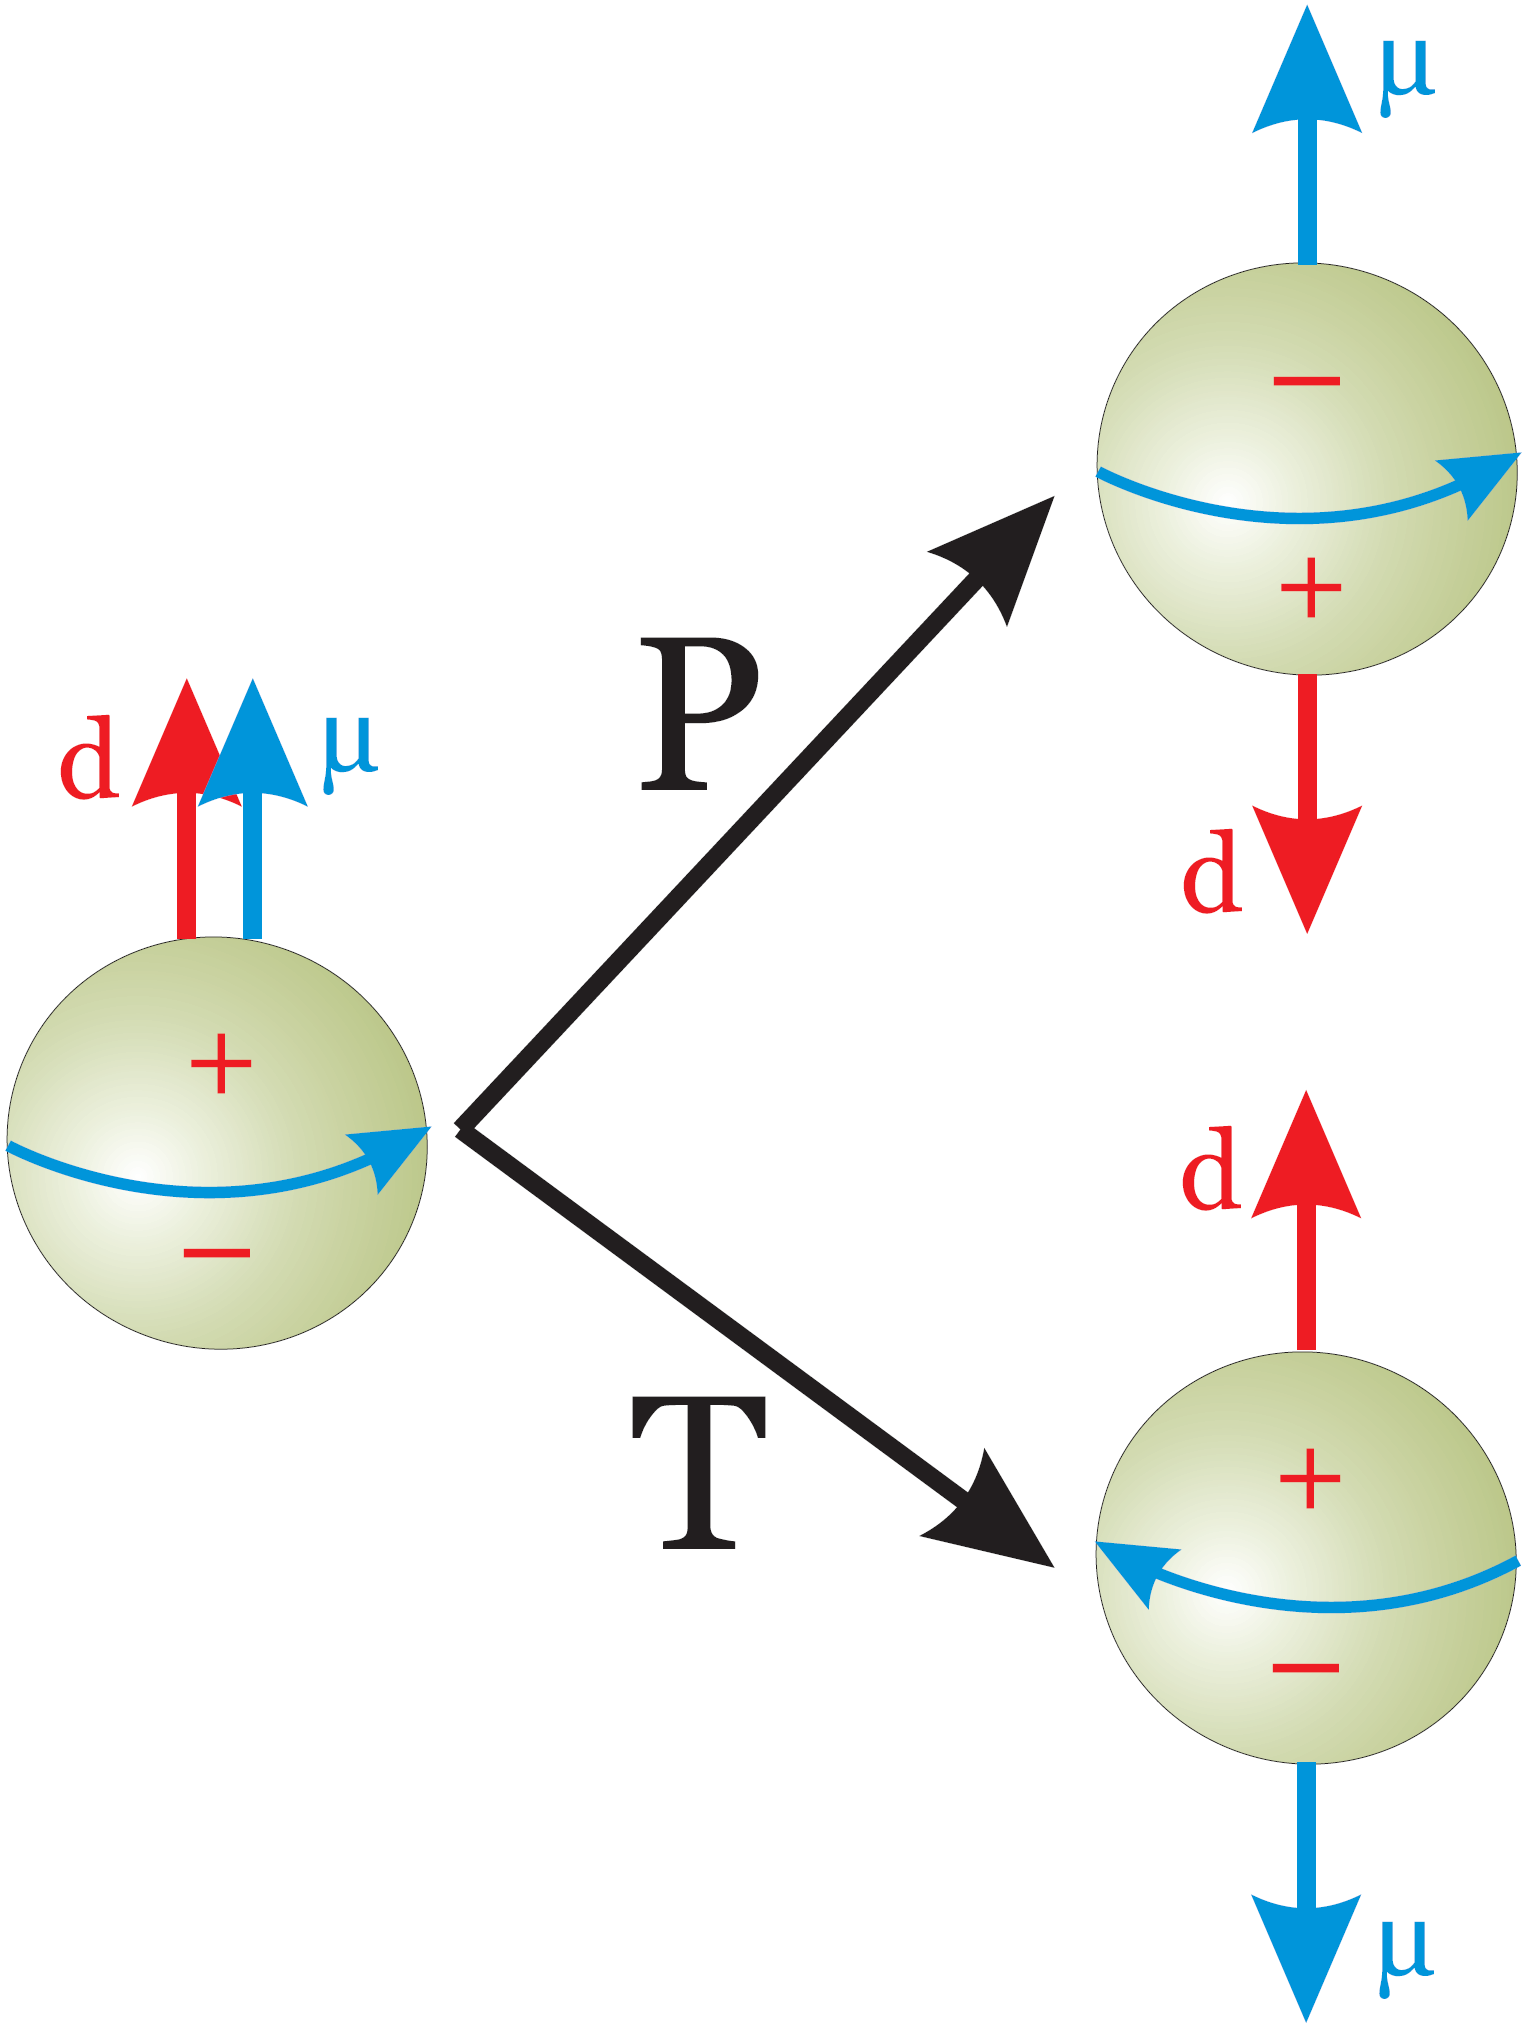
\includegraphics[width=0.4\linewidth]{images/4_EDM_P_T}
	\caption{Схематическое изображение нарушение P- и Т-симметрии ненулевым электрическим дипольным моментом.}
	\label{fig:4edmpt}
\end{figure}

\par	Исследование ЭДМ осуществляется, согласно уравнению Т-БМТ, по его влиянию на поведение поляризации в электромагнитных полях. Для нейтрона и нейтральных атомов поляризация сохраняется при воздействии внешних магнитных и электрических полей. В случае заряженных частиц движение определяется силой Лоренца, что требует применения ускорительных установок, обеспечивающих длительное накопление пучка с заданными параметрами и выполняющих роль накопительного кольца. Наиболее перспективным направлением является изучение ЭДМ протона и дейтрона. Для этого создаются поляризованные пучки с максимально близкими свойствами в плане прецессии спина во внешних полях. Это позволяет сохранять поляризацию вдоль выбранной оси, при этом спины частиц прецессируют с одинаковой частотой. Для измерения величины ЭДМ на уровне $10^{-29}$ $e\cdot \text{см}$ необходимо удерживать пучок на орбите с сохранением поляризации в течение времени порядка $\sim1000$ с, с последующим анализом рассеяния на мишени поляриметра. Влияние магнитного дипольного момента (МДМ) при этом должно быть подавлено до величины, меньшей сигнала ЭДМ. Такая техника впервые была предложена в Брукхейвенская Национальная Лаборатория (BNL) и получила название "\textit{замороженный спин}" \autocite{Farley:edm}. Позднее была предложена концепция "\textit{квази-замороженного спина}" \autocite{QFS}, в которой осуществляется пространственное разделение электрического и магнитного полей, а условия подавления влияния МДМ выполняются за полный оборот по кольцу.

\par	Ещё одним перспективным направлением исследований в рамках программы спиновой физики является поиск аксионоподобных частиц. Изучается резонанс, возникающий при совпадении $g-2$ частоты прецессии спина вокруг ведущего магнитного поля ускорителя с частотой колебаний аксионного поля. В этом случае ускоритель выполняет роль широкополосной зондирующей антенны по частоте спиновой прецессии \autocite{Axion_Nikolaev}.

\par	Приведённые вопросы фундаментальной физики требуют детального изучения и исследуются с помощью ускорительных установок. Такие установки обеспечивают достижение высоких энергий частиц и предельной точности измерений. Практика использования подобных комплексов распространена в мировых ядерных центрах: CERN \autocite{lhc:heavy_ions}, BNL \autocite{rhic:design}, J-PARC \autocite{j-park}. 

\par	Ускорительный комплекс NICA (Nuclotron-based Ion Collider fAсility) является современным центром, оснащённым передовой материально-технической базой и формируемым на базе ОИЯИ в городе Дубна, Россия \autocite{nuclotron24}. Основной установкой комплекса является коллайдер, в котором предусмотрены два места встречи пучков, где расположены два детектора: MPD (Multi-Purpose Detector) и SPD (Spin Physics Detector) \autocite{Ladygin:SPD}. Каждый из этих детекторов предназначен для проведения различных экспериментов. MPD-детектор используется для исследования кварк-глюонной плазмы, возникающей в результате столкновения тяжёлых ионов \autocite{Tech, MPD}. SPD-детектор направлен на изучение поведения сталкивающихся поляризованных пучков протонов и дейтронов. Кинематическая область, охватываемая SPD, уникальна и ранее не применялась для целенаправленных исследований поляризованных адронных столкновений. Особый интерес представляет возможность изучения поляризованных дейтронов. Таким образом, структура коллайдера должна обеспечивать ускорение как тяжёлых ионов, так и лёгких частиц, при этом требования к удержанию пучков различаются в зависимости от типа частиц.

\par Исследования направлены на расширение существующей физической программы, дополняя её новым направлением исследований с поляризованными пучками. В работе ускоритель выступает как экспериментальная установка, позволяя исследовать процессы в пучке непосредственно в комплексе Nuclotron-NICA. Предложенные подходы применимы также на других аналогичных установках без потери общности.
~\\
\par {\aim} данной диссертации является изучение особенностей поведения тяжёлых ионов и поляризованных пучков лёгких заряженных частиц в предлагаемой дуальной структуре, а также исследования электрического дипольного момента с использованием квази-замороженной концепции.
Для достижения поставленной цели необходимо было решить следующие {\tasks}:
\begin{enumerate}[beginpenalty=10000] % https://tex.stackexchange.com/a/476052/104425
	\item	Определить требования к дуальной структуре для работы с тяжёлыми ионами и лёгкими частицами;
	\item	Регулировать критическую энергии для поляризованного пучка в резонансной структуре;
	\item	Провести численное моделирование динамики пучка лёгких частиц с учётом высших порядков коэффициента уплотнения орбиты в высокочастотных резонаторах гармонического и барьерного типов;
	\item 	Изучить поведение динамической апертуры с учетом высших порядков при прохождении пучка через критическую энергию и компенсации хроматичности;
	\item 	Определить особенности поведения поляризации пучка при пересечении критической энергии;
	\item 	Исследовать концепцию «квази-замороженного» спина с целью создания установки для изучения ЭДМ протона и дейтрона;
	\item	Исследовать спин-орбитальное движение поляризованного пучка в магнитном кольце с фильтрами Вина.
\end{enumerate}
~\\
\par {\novelty}
\begin{enumerate}[beginpenalty=10000] % https://tex.stackexchange.com/a/476052/104425
	\item	Впервые предложена дуальная структура для тяжёлых ионов и лёгких частиц для коллайдера NICA;
	\item 	Впервые предложены методы подавления дисперсии поворотной аркой в резонансной магнитооптической структуре с отсутствующими магнитами;
	\item 	Впервые исследован метод скачка критической энергии с использованием барьерного ускоряющего потенциала с учётом ограничений по продольной микроволновой неустойчивости;
	\item	Проведено исследование продольной динамики с учётом высших порядков разложения по импульсу и влияния импеданса; на его основе сформулированы ограничения на величину и темп скачка критической энергии исследуемого кольца;
	\item	Разработаны 8- и 16-периодичные квази-замороженные структуры Nuclotron для выделения ЭДМ сигнала лёгких ядер;
	\item	Создана структура коллайдера NICA с обводными каналами, изначально не ориентированная на эксперименты по поиску ЭДМ дейтрона методом квази-замороженного спина.
\end{enumerate}
~\\
\par {\influence}:
\par	Проведённый анализ динамики пучка вблизи критической энергии позволил определить её влияние на устойчивость движения поляризованных протонных пучков и установить оптимальные параметры процедуры её преодоления.

\par	Разработанная дуальная структура обеспечивает эффективную работу как с тяжёлыми ионами, так и с лёгкими частицами, что делает возможным проведение двух направлений исследований в одном ускорительном комплексе: экспериментов по изучению кварк-глюонной плазмы и исследований поляризованных пучков в симметричных и асимметричных коллайдерных режимах.

\par Расширена применимость метода резонансных структур для случаев с нарушенной периодичностью дисперсионной функции на арках.

\par Для поляризованных частиц адаптирован метод «квази-замороженного спина» к условиям коллайдера NICA. Разработана магнитооптическая схема обводных каналов с фильтрами Вина, обеспечивающая реализацию экспериментов по измерению электрического дипольного момента дейтрона без существенной модификации базовой структуры ускорителя. 

\par Предложенные решения могут быть использованы не только на NICA, но и на Nuclotron с сохранением функций бустера для поляризованных пучков, что создаёт возможность проведения независимых экспериментов по поиску ЭДМ и аксиона в рамках программы спиновой физики комплекса NICA–Nuclotron.

%\par {\progress}
%Разработанность темы ТАКАЯ
%~\\

\par {\methods} Основными методами исследования являются математическое и компьютерное моделирование, численный эксперимент. Для исследования были использованы программы для расчёта поперечной динамики: MAD-X \autocite{madx}, OPTIM \autocite{optim}, BMAD \autocite{bmad}, продольной динамики: BLonD \autocite{blond}, спин-орбитальной динамики: COSY Infinity \autocite{cosy}.
~\\

\par {\defpositions}
\begin{enumerate}[beginpenalty=10000] % https://tex.stackexchange.com/a/476052/104425
	\item 	Предложена дуальная структура комплекса NICA–Nuclotron, оптимизированная для тяжёлых ионов с учётом внутрипучкового рассеяния и для лёгких частиц с повышенной критической энергией, превышающей энергию эксперимента; \autocite{Kolokolchikov:2025_dual, Syresin:2021_polar}
	\item	Реализован метод резонансной магнитооптической структуры с отсутствующими магнитами и подавлением дисперсии двумя семействами квадруполей и крайними ячейками поворотной арки; \autocite{Kolokolchikov:2021trans, Kolokolchikov:2023_pecular}
	\item	Выполнено численное моделирование продольной динамики протонного поляризованного пучка с учётом высших порядков по импульсу и продольных импедансов вблизи критической энергии; результаты сопоставлены с экспериментами на ускорителе У-70; \autocite{Kolokolchikov:2025_U70, Kolokolchikov:2025_jump}
	\item 	Проведён анализ использования гармонического и барьерного ВЧ при скачке критической энергии; для барьерного ВЧ показана возможность сокращения расстояния между барьерами с учётом продольной микроволновой неустойчивости; \autocite{Kolokolchikov:2024_bb_rupac, Kolokolchikov:2023_bb_IPAC, Kolokolchikov:2024_bb_dspin}
	\item	Предложены модернизированные 8- и 16-периодные структуры Nuclotron с квази-замороженным спином для экспериментов по измерению ЭДМ лёгких ядер при сохранении функций бустера; \autocite{Senichev:2023_QFS, Senichev:2023_nuclotron, Kolokolchikov:2025_nuclotron}
	\item	Применён метод фильтров Вина для сохранения поляризации и выделения ЭДМ-сигнала в пучке дейтронов, реализованный в структуре коллайдера NICA с введением обводных каналов.; \autocite{Kolokolchikov:2023_bypass_ru, Kolokolchikov:2023_bypass_IPAC, Senichev:2024_nica_edm, Kolokolchikov:2023_sc, Kolokolchikov:2023_sc_IPAC}
\end{enumerate}

~\\
\par {\reliability} полученных результатов подтверждается согласованием аналитических вычислений с результатами численных экспериментов. Результаты находятся в соответствии с результатами, полученными другими авторами.
~\\
\par {\probation}
Основные результаты работы были представлены~на российских и международных конференциях, а также были представлены на рабочих встречах: 
\begin{itemize}
\item Workshop “Polarized beam in NICA” в 2022 г.;
\item Молодежная конференция по теоретической и экспериментальной физике МКТЭФ-2020. Москва, Россия;
\item 63, 65, 66-ая Всероссийская научная конференция МФТИ в 2020, 2023, 2024 гг. г. Долгопрудный,
Россия;
\item XXVII и XXVIII Всероссийская конференции по ускорителям заряженных частиц RuPAC'21, RuPAC'23. Алушта; Новосибирск, Россия;
\item VII, VIII, IX и X Международная конференция Лазерные и Плазменные технологии ЛаПлаз'21, ЛаПлаз'22, ЛаПлаз'23, ЛаПлаз'24, ЛаПлас'25. Москва, Россия;
\item XIII, XIV, XVI международная конференция по ускорителям заряженных частиц IPAC'22 IPAC'23, IPAC'25. Бангкок, Тайланд; Венеция, Италия; Тайпей, Тайвань;
\item XIX Международная конференции по спиновой физике высоких энергий DSPIN'23. Дубна, Россия;
\item XI-я Международная конференция по ядерной физике в накопительных кольцах STORI’24. Хуэйчжоу, провинция Гуандун, Китай;
\end{itemize}
~\\
\par {\contribution} Все результаты, выносимые на защиту, получены автором лично, либо при его непосредственном участии. Содержание диссертации и выносимые на защиту основные положения отражают личный вклад автора в опубликованные работы. Результаты по подготовке и проведению эксперимента на ускорителе У-70 получены в соавторстве с сотрудниками ИЯИ РАН и ИФВЭ. Подготовка к публикации полученных результатов проводилась совместно с соавторами.
~\\

\par \ifnumequal{\value{bibliosel}}{0}
{%%% Встроенная реализация с загрузкой файла через движок bibtex8. (При желании, внутри можно использовать обычные ссылки, наподобие `\autocite{vakbib1,vakbib2}`).
	{\publications} Основные результаты по теме диссертации изложены
	в~XX~печатных изданиях,
	X из которых изданы в журналах, рекомендованных ВАК,
	X "--- в тезисах докладов.
}%
{%%% Реализация пакетом biblatex через движок biber
	\begin{refsection}[bl-author, bl-registered]
		% Это refsection=1.
		% Процитированные здесь работы:
		%  * подсчитываются, для автоматического составления фразы "Основные результаты ..."
		%  * попадают в авторскую библиографию, при usefootcite==0 и стиле `\insertbiblioauthor` или `\insertbiblioauthorgrouped`
		%  * нумеруются там в зависимости от порядка команд `\printbibliography` в этом разделе.
		%  * при использовании `\insertbiblioauthorgrouped`, порядок команд `\printbibliography` в нём должен быть тем же (см. biblio/biblatex.tex)
		%
		% Невидимый библиографический список для подсчёта количества публикаций:
		\printbibliography[heading=nobibheading, section=1, env=countauthorvak,          keyword=biblioauthorvak]%
		\printbibliography[heading=nobibheading, section=1, env=countauthorwos,          keyword=biblioauthorwos]%
		\printbibliography[heading=nobibheading, section=1, env=countauthorscopus,       keyword=biblioauthorscopus]%
		\printbibliography[heading=nobibheading, section=1, env=countauthorconf,         keyword=biblioauthorconf]%
		\printbibliography[heading=nobibheading, section=1, env=countauthorother,        keyword=biblioauthorother]%
		\printbibliography[heading=nobibheading, section=1, env=countregistered,         keyword=biblioregistered]%
		\printbibliography[heading=nobibheading, section=1, env=countauthorpatent,       keyword=biblioauthorpatent]%
		\printbibliography[heading=nobibheading, section=1, env=countauthorprogram,      keyword=biblioauthorprogram]%
		\printbibliography[heading=nobibheading, section=1, env=countauthor,             keyword=biblioauthor]%
		\printbibliography[heading=nobibheading, section=1, env=countauthorvakscopuswos, filter=vakscopuswos]%
		\printbibliography[heading=nobibheading, section=1, env=countauthorscopuswos,    filter=scopuswos]%
		%
		\nocite{*}%
		%
		{\publications} Основные результаты по теме диссертации изложены в~\arabic{citeauthor}~печатных изданиях, 13 из которых изданы в журналах, рекомендованных ВАК\sloppy%
		\ifnum \value{citeauthorscopuswos}>0%
		, \arabic{citeauthorscopuswos} "--- в~периодических научных журналах, индексируемых Web of~Science и Scopus\sloppy%
		\fi%
		\ifnum \value{citeauthorconf}>0%
		, \arabic{citeauthorconf} "--- в~тезисах докладов.
		\else%
		.
		\fi%
		\ifnum \value{citeregistered}=1%
		\ifnum \value{citeauthorpatent}=1%
		Зарегистрирован \arabic{citeauthorpatent} патент.
		\fi%
		\ifnum \value{citeauthorprogram}=1%
		Зарегистрирована \arabic{citeauthorprogram} программа для ЭВМ.
		\fi%
		\fi%
		\ifnum \value{citeregistered}>1%
		Зарегистрированы\ %
		\ifnum \value{citeauthorpatent}>0%
		\formbytotal{citeauthorpatent}{патент}{}{а}{}\sloppy%
		\ifnum \value{citeauthorprogram}=0 . \else \ и~\fi%
		\fi%
		\ifnum \value{citeauthorprogram}>0%
		\formbytotal{citeauthorprogram}{программ}{а}{ы}{} для ЭВМ.
		\fi%
		\fi%
		% К публикациям, в которых излагаются основные научные результаты диссертации на соискание учёной
		% степени, в рецензируемых изданиях приравниваются патенты на изобретения, патенты (свидетельства) на
		% полезную модель, патенты на промышленный образец, патенты на селекционные достижения, свидетельства
		% на программу для электронных вычислительных машин, базу данных, топологию интегральных микросхем,
		% зарегистрированные в установленном порядке.(в ред. Постановления Правительства РФ от 21.04.2016 N 335)
	\end{refsection}%
	\begin{refsection}[bl-author, bl-registered]
		% Это refsection=2.
		% Процитированные здесь работы:
		%  * попадают в авторскую библиографию, при usefootcite==0 и стиле `\insertbiblioauthorimportant`.
		%  * ни на что не влияют в противном случае
		%\nocite{vakbib2}%vak
		%\nocite{patbib1}%patent
		%\nocite{progbib1}%program
		%\nocite{bib1}%other
		%\nocite{confbib1}%conf
	\end{refsection}%
	%
	% Всё, что вне этих двух refsection, это refsection=0,
	%  * для диссертации - это нормальные ссылки, попадающие в обычную библиографию
	%  * для автореферата:
	%     * при usefootcite==0, ссылка корректно сработает только для источника из `external.bib`. Для своих работ --- напечатает "[0]" (и даже Warning не вылезет).
	%     * при usefootcite==1, ссылка сработает нормально. В авторской библиографии будут только процитированные в refsection=0 работы.
}
